In chapters~\ref{ch:mvica1},~\ref{ch:mvica2},~\ref{ch:shica} and
\ref{ch:shica2}, we have used ICA-based methods to learn shared responses from different
subjects performing the same task.
In this chapter we present an ICA-based method to achieve data augmentation for fMRI data.

  Advances in computational cognitive neuroimaging research are
  related to the availability of large amounts of labeled brain
imaging data, since classifiers used to decode brain maps have large
sample-complexity.
%
However such data are scarce.
%

To tackle this problem, data generation is an attractive approach, as
it could potentially compensate for the shortage of data.
Conditional Generative Adversarial Networks (CGANs) are promising generative
models~\cite{goodfellow2014generative} designed for computer vision.
% 
However, such improvements have not yet carried over to brain imaging. A likely
reason is that CGANs are ill-suited to the noisy, high-dimensional and
small-sample data available in functional neuroimaging. 
% 
Furthermore the training of CGANs is notoriously unstable and there are many hyper-parameters to tune.
% 

  In this work, we introduce Conditional ICA: a novel data augmentation technique using ICA together with conditioning mechanisms to generate surrogate brain imaging data and improve image classification performance.
  % 
  Conditional ICA benefits from the abundant
  resting state data and can be trained with only few labeled samples.


%
\begin{figure}
\centerline{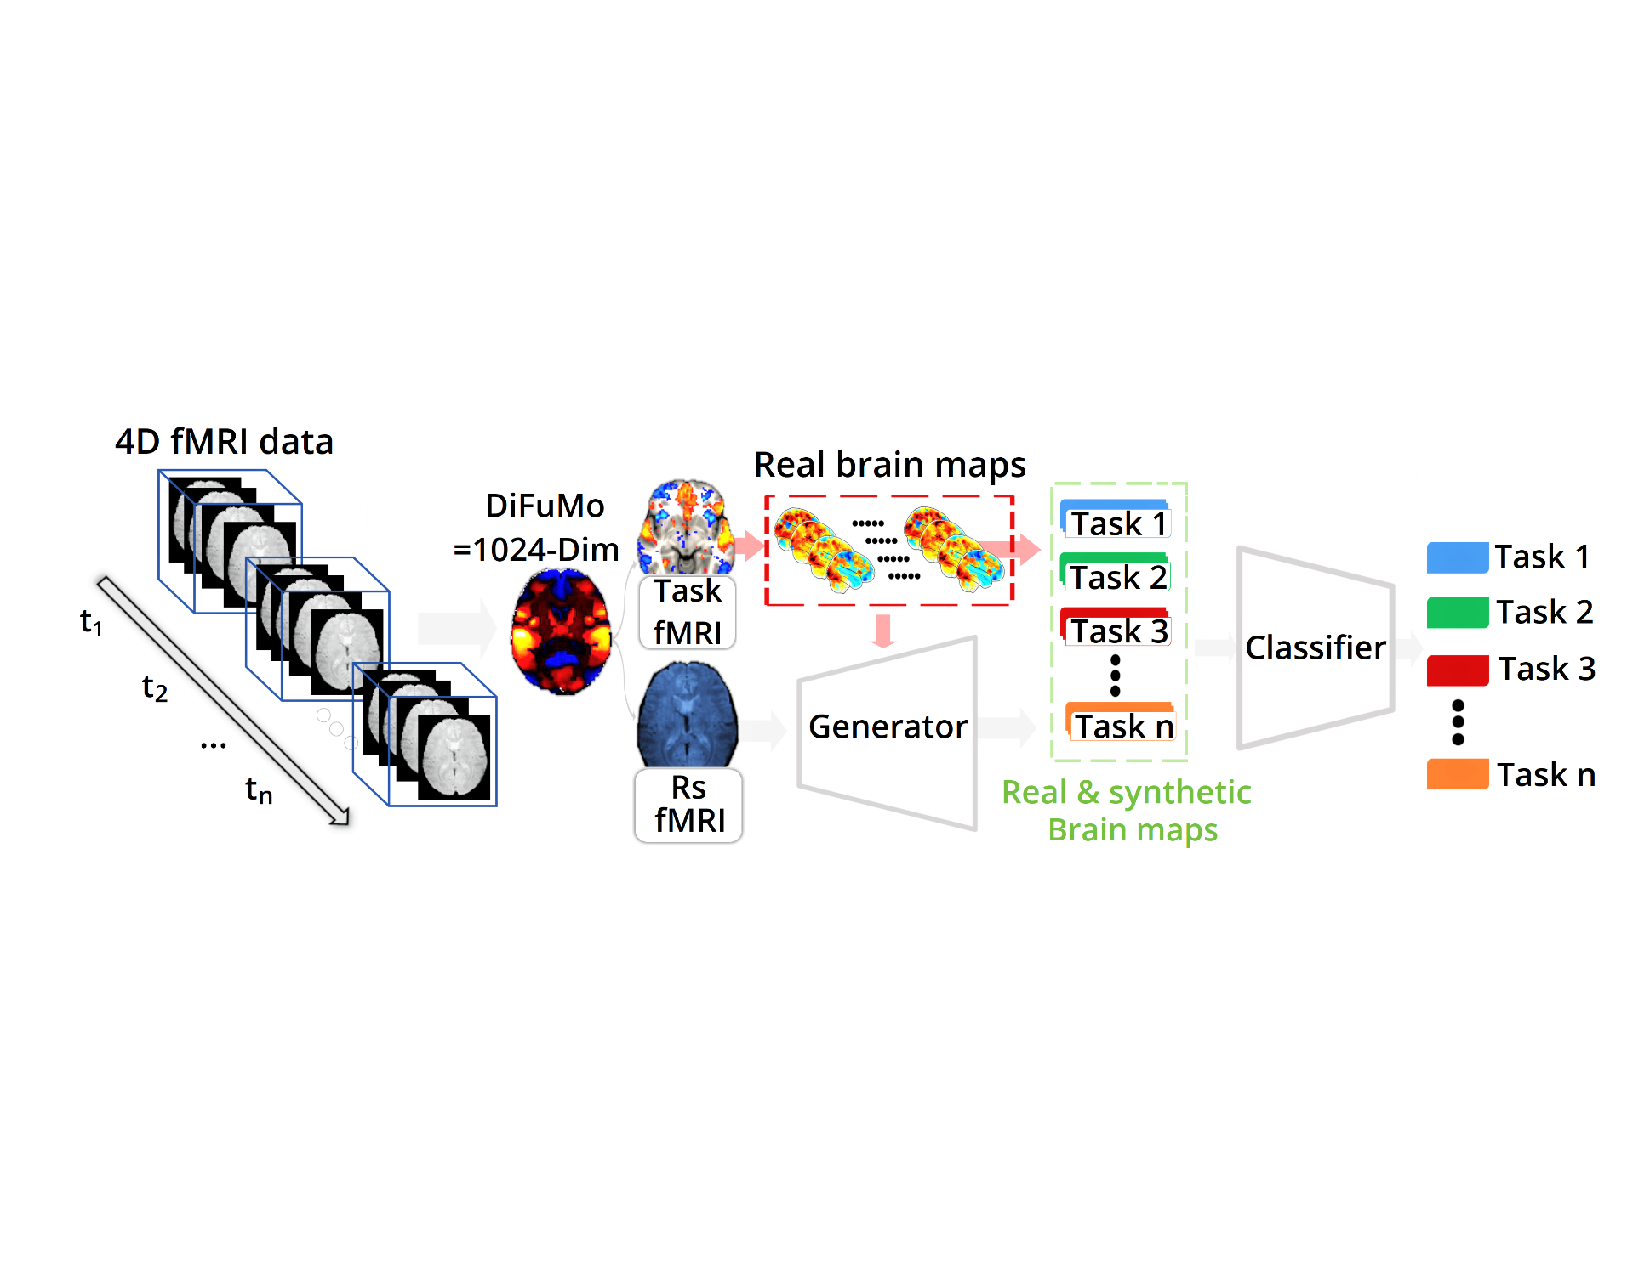
\includegraphics[width=1\textwidth]{condica/conceptual_figure_1_v6_redim.pdf}}
\caption{\textbf{Conditional ICA approach.} Our method aims to
  generate surrogate data from Task and Rest fMRI data by synthesizing
  statistical maps that qualitatively fit the distribution of the
  original maps. These can be used to improve the accuracy of
  machine learning models that identify contrasts from the
  corresponding brain activity patterns.}
\label{Fig0}
\end{figure}



\section{Methods}

\subsection{Spatial Dimension reduction.} 
The outline of the proposed approach is presented in Fig.\ref{Fig0}.
%
While brain maps are high-dimensional, they span a smaller space than that of
the voxel grid. 
%
For the sake of tractability, we reduce the dimension of the data by projecting the voxel values on the
high-resolution version of the Dictionaries of Functional Modes \emph{DiFuMo}
atlas \cite{dadi_fine-grain_2020}, i.e. with $p=1024$ components.
%
The choice of dimension reduction technique generally has an impact on the
results. However we consider this question to be out of the scope of the current study and leave this to future work.

\subsection{A generative model for task data}
Consider a task dataset $X^{task}$ in $\mathbb{R}^{p,n}$ where $n$ is the number of observations
(samples) and $p=1024$ the number of components in the atlas. $X^{task}$ can be seen as $n$
observations of a random vector $\xb^{task} \in \RR^p$. Let us
consider how to learn the distribution of $\xb^{task}$. 
%
Assuming a Gaussian distribution is standard in this setting, yet, as
shown later, it misses key distributional features.
%
Moreover, we consider a model that subsumes the distribution of any type of
fMRI data (task or rest): a linear mixture of $k \leq p$ independent temporal signals.
%
We therefore use temporal ICA to learn a dimension reduction and unmixing matrix
$W^{task} \in \mathbb{R}^{k, p}$ such that the $k$ components i.e the $k$ components of
$W^{task} \xb^{task}$ are as
independent as possible.

A straightforward method to generate new task data would be to
independently sample them from the distribution of the components.
%
This is easy because such distribution has supposedly independent marginals.
We apply an invertible quantile transform $q^{task}$ to the components of $W^{task} \xb^{task}$ so that
the distribution of $q^{task}(W^{task} \xb^{task})$ has standardized Gaussian
marginals. Since it also has independent marginals it is given by $\mathcal{N}(\zero_k, I_k)$
from which we can easily sample.

However task datasets   have a small number of samples ($10 \sim 10^2$). As a
result, there are too few samples to learn high quality unmixing matrices. In
contrast, resting state datasets have a large number of samples ($10^4 \sim 10^5$).
Therefore we replace the unmixing matrix learned on task data $W^{task}$ by the
unmixing matrix learned on resting state data $W^{rest}$.

We form $\zb^{task} = W^{rest} \xb^{task}$ and learn its quantile
transform $q$.
The encoding model is thus given by:
\begin{align}
  \zb^{task} = q(W^{rest} \xb^{task})
\end{align}

However, the independence assumption no longer holds and thus a latent structure among the marginals of
$\zb^{task}$ has to be taken into account. In addition the generative model needs
to be conditioned to each class. We therefore assume that the samples in class
$c$, $\xb_c^{task}$ are such that:
\begin{align}
q(W^{rest}\xb^{task}_c) \sim \Ncal( \mu_c, \Lambda)
\end{align}

In order to maximize the number of samples used to learn the parameters of the
model, we assume that the quantile transform $q$ and the latent covariance
$\Lambda$ do not depend on the class $c$. However, the mean $\mub_c$, that can be learned efficiently using just a few tens of samples, depends on class $c$.
$\Lambda$ is learned using all task samples from a standard shrunk covariance
estimator
$\Lambda = \Sigma (1 - \alpha) + \frac{\alpha}{k} \tr(\Sigma) I_k$ where
$\alpha$ is given by the Ledoit-Wolf formula \cite{ledoit2004well} and
$\Sigma$ is the sample covariance of $\zb^{task}$.

The generative model of data for brain maps in a certain class $c$ is given by the pseudo inverse of the encoding model:
\begin{equation}
  \xb_c = (W^{rest})^{\dagger} q^{-1}(\epsilonb)
\end{equation}
with $\epsilonb \sim \mathcal{N}(\mub_c, \Lambda)$ and $(W^{rest})^{\dagger}$ is
the Moore Penrose inverse of $W^{rest}$

An overview of our generative method is shown in Fig.~\ref{Fig11}.
%
\begin{figure}
\centerline{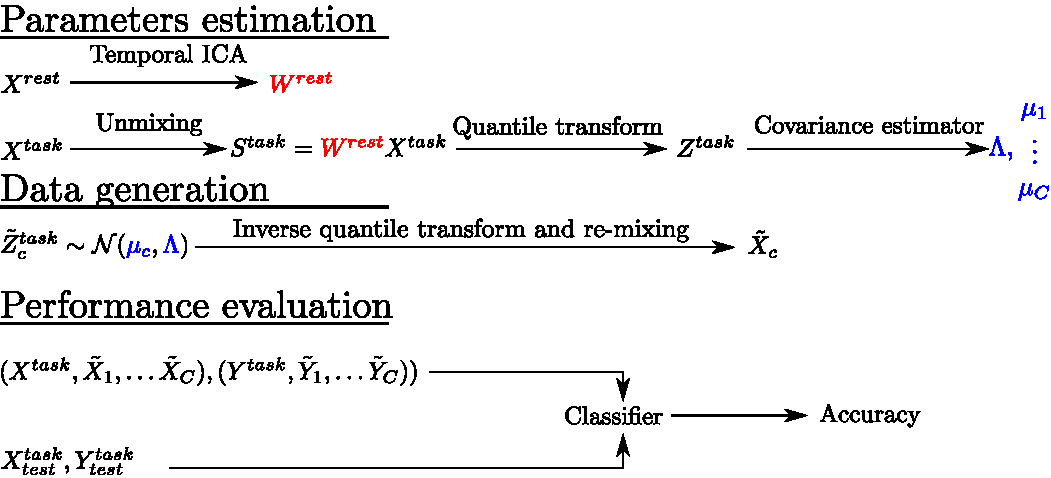
\includegraphics[width=1\textwidth]{figures/condica/method_figure}}
\caption{\textbf{Conditional ICA approach in depth.} 
The approach proceeds by learning a temporal ICA of rest data $X^{rest} \in
\mathbb{R}^{p, n}$ , resulting in
independent components and unmixing matrix $W^{rest} \in \mathbb{R}^{k, p}$.
%
Applying the unmixing matrix to the task data, we obtain samples in the component
space that we map to a normal distribution, yielding $Z^{task} \in
\mathbb{R}^{k, n}$. 
%
Then, we estimate the covariance $\Lambda \in \mathbb{R}^{k, k}$ (all classes are assumed to have the
same covariance) and the class-specific means $\boldsymbol{\mu}_1, \dots, \mub_C \in \mathbb{R}^{k}$ according to Ledoit-Wolf's method.
%
For each class $c$, we can draw random samples $\tilde{Z}^{task}_c \in
\mathbb{R}^{k, n_{\mathrm{fakes}}}$ from the
resulting multivariate Gaussian distribution $\mathcal{N}(\mub_c, \Lambda)$ and
obtain fake data $\tilde{X}_c  \in
\mathbb{R}^{p, n_{\mathrm{fakes}}}$
by applying the inverse quantile transform and re-mixing the data using the pseudo inverse of the unmixing matrix.
%
We append these synthetic data to the actual data to create our new augmented
dataset on which we train classifiers.}
\label{Fig11}
\end{figure}
%

\section{Related work}
In image processing, data augmentation is part of standard toolboxes and
typically includes operations like cropping, rotation, translation.
%
On fMRI data these methods do not make much sense as brain data are not invariant to such transformations.
%
More advanced techniques~\cite{zhuang2019fmri} %\cite{sandfort2019data}
are based on generative models such as CGANs or variatonal
auto-encoders~\cite{kingma2013auto}. Although CGAN-based method are powerful they are slow and difficult to train~\cite{arjovsky_wasserstein_2017}.

Our method is not an adversarial procedure, however it relates to other
powerful generative models such as variatonal
auto-encoders~\cite{kingma2013auto} with which it shares strong similarities.
Indeed the analog of the encoding function in the variational auto-encoder is
given by $e(\xb) = \Lambda^{-\frac12}q(W^{rest} \xb)$ in our model and the analog to the decoding
function in the variational auto-encoder is given by $d(\zb) =
(W^{rest})^{\dagger}q^{-1}(\Lambda^{\frac12}\zb)$ in our model. As in the variational auto-encoder, $e$ approximately maps the empirical data distribution to a standardized Gaussian distribution,
while the reconstruction error defined by the difference in l2 norm
$\|d(e(\xb)) - \xb\|^2_2$ must remain small.
Lastly, another classical generative model related to ours is normalizing
flows.  We note that when $W^{rest}$ is square (no dimension reduction in ICA), the decoding operator $d$ is invertible (its inverse is $e$) making our
model an instance of normalizing flows~\cite{rezende2015variational}. 
%
A great property is thus the simplicity and reduced cost of data generation.

\section{Conclusion}
In this chapter, we introduced Conditional ICA, a fast generative model for task
data.
Conditional ICA is essentially a linear generative model with
pointwise non-linearity, which makes it cheap, easy to instantiate on new data,
and to introspect.
In the next chapter, we look at the performance of Conditional ICA on fMRI data.

